\documentclass[a4paper, 11pt]{article}
\usepackage{graphicx}
\usepackage[utf8]{vietnam}
\usepackage{indentfirst}
\usepackage{longtable}
\usepackage{fdsymbol}
\usepackage{color}
\usepackage{biblatex}
\usepackage{fullpage}
\usepackage{blindtext}
\usepackage{hyperref}
\usepackage{multicol}
\usepackage{caption}
\usepackage{amsmath}
\usepackage[table]{xcolor}
\usepackage{geometry}
\usepackage{listings}

\definecolor{codegreen}{rgb}{0,0.6,0}
\definecolor{codegray}{rgb}{0.5,0.5,0.5}
\definecolor{codepurple}{rgb}{0.58,0,0.82}
\definecolor{backcolour}{rgb}{0.95,0.95,0.92}

\lstdefinestyle{mystyle}{
    backgroundcolor=\color{backcolour},
    commentstyle=\color{codegreen},
    keywordstyle=\color{magenta},
    numberstyle=\tiny\color{codegray},
    stringstyle=\color{codepurple},
    basicstyle=\ttfamily\footnotesize,
    breakatwhitespace=false,
    breaklines=true,
    captionpos=b,
    keepspaces=true,
    numbers=left,
    numbersep=5pt,
    showspaces=false,
    showstringspaces=false,
    showtabs=false,
    tabsize=4
}

\lstset{style=mystyle}

\setcounter{MaxMatrixCols}{20}

\title{Bài tập tổng hợp cuối kỳ môn quản trị hệ thống}
\author{Kim Minh Thắng B2007210}

\begin{document}
\maketitle
\tableofcontents
\listoffigures
\listoftables
\lstlistoflistings

\section*{Mô tả bài tập}

Công ty Straw Hat chuyên kinh doanh hải sản có nhu cầu xây dựng hệ thống mạng cục bộ phục vụ cho công việc của công ty như sau:

\begin{minipage}{\linewidth}
    \captionsetup{type=figure}
    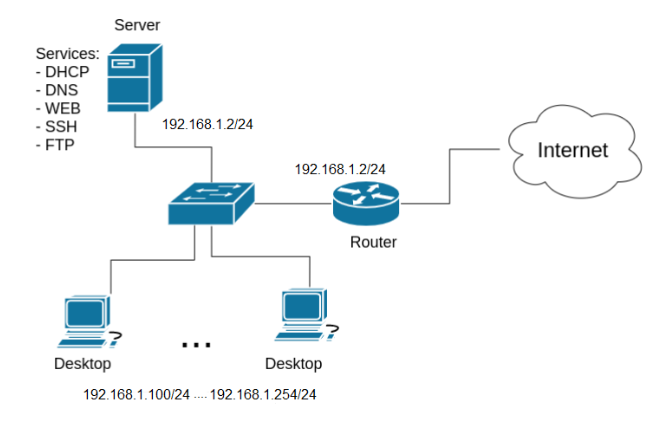
\includegraphics[width=12cm]{images/networks.png}
    \caption{Sơ đồ hệ thống mạng của công ty Straw Hat}
\end{minipage}

\section{Cài đặt và cấu hình Server/Desktop}

\subsection{(10\%) Sử dụng phần mềm VirtualBox cài đặt Server và Desktop:}

\begin{itemize}
    \item Tạo 1 NAT Network tên "QTHT" có địa chỉ mạng là 192.168.1.0/24. Tắt dịch vụ DHCP có sẵn trên NAT Network "QTHT". \hfill \\
          \begin{minipage}{\linewidth}
              \captionsetup{type=figure}
              \centering
              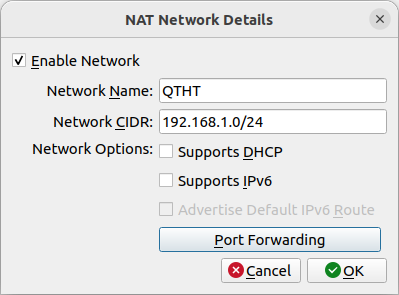
\includegraphics[width=8cm]{images/create-nat.png}
              \caption{Cấu hình NAT Network QTHT}
          \end{minipage}

          Để tắt dịch vụ DHCP mặc định của NAT Network trong VirtualBox, ta bỏ tích tùy chọn "Supports DHCP".

    \item Tạo 2 máy ảo với thông tin như sau: \hfill \\
          \begin{minipage}{\linewidth}
              \begin{multicols}{2}
                  \begin{minipage}{\linewidth}
                      \captionsetup{type=table}
                      \caption{Cấu hình máy Server}
                      \centering
                      \begin{tabular}{| p{.3\linewidth} | p{.4\linewidth} |}
                          \hline
                          \textbf{Hostname}         & Server                                                               \\
                          \hline

                          \textbf{Hệ điều hành}     & CentOS 9                                                             \\
                          \hline

                          \textbf{CPU / RAM / DISK} & 1core/2G/10G \newline Hoặc tùy chỉnh theo cấu hình máy của sinh viên \\
                          \hline

                          \textbf{Network}          & NAT Network \newline Name: "QTHT"                                    \\
                          \hline

                          \textbf{IP}               & 192.168.1.2                                                          \\
                          \hline

                          \textbf{Subnet mask}      & 255.255.255.0                                                        \\
                          \hline

                          \textbf{Gateway}          & 192.168.1.1                                                          \\
                          \hline

                          \textbf{DNS}              & 192.168.1.1                                                          \\
                          \hline
                      \end{tabular}
                  \end{minipage}

                  \begin{minipage}{\linewidth}
                      \captionsetup{type=table}
                      \caption{Cấu hình máy Desktop}
                      \centering
                      \begin{tabular}{| p{.3\linewidth} | p{.4\linewidth} |}
                          \hline
                          \textbf{Hostname}                                              & Desktop                                                              \\
                          \hline

                          \textbf{Hệ điều hành}                                          & Lubuntu 22.04, \newline hoặc bất kỳ hệ điều hành khác                \\
                          \hline

                          \textbf{CPU / RAM / DISK}                                      & 1core/2G/10G \newline Hoặc tùy chỉnh theo cấu hình máy của sinh viên \\
                          \hline

                          \textbf{Network}                                               & NAT Network \newline Name: "QTHT"                                    \\
                          \hline

                          \textbf{IP \newline Subnet mask \newline Gateway \newline DNS} & Cấu hình tự động sử dụng dịch vụ DHCP                                \\
                          \hline
                      \end{tabular}
                  \end{minipage}
              \end{multicols}
          \end{minipage}
          \begin{enumerate}
              \item \textbf{Server có cấu hình như sau:}
                    \begin{itemize}
                        \item Hệ điều hành: CentOS 9
                        \item CPU: 1 Core \textit{(Hình \ref{figure:server-processor})}
                        \item Ram: 4GB \textit{(Hình \ref{figure:server-ram})}
                        \item Disk: 20GB \textit{(Hình \ref{figure:server-disk})}
                        \item Network: NAT Network "QTHT" \textit{(Hình \ref{figure:server-network-1})}
                        \item IPv4: 192.168.1.2 \textit{(Hình \ref{figure:server-network-2})}
                        \item Subnet mask: 255.255.255.0 \textit{(Hình \ref{figure:server-network-2})}
                        \item Gateway: 192.168.1.1 \textit{(Hình \ref{figure:server-network-2})}
                        \item DNS: 192.168.1.1 \textit{(Hình \ref{figure:server-network-2})}
                    \end{itemize}

                    \begin{minipage}
                        {\linewidth}
                        \captionsetup{type=figure}
                        \centering
                        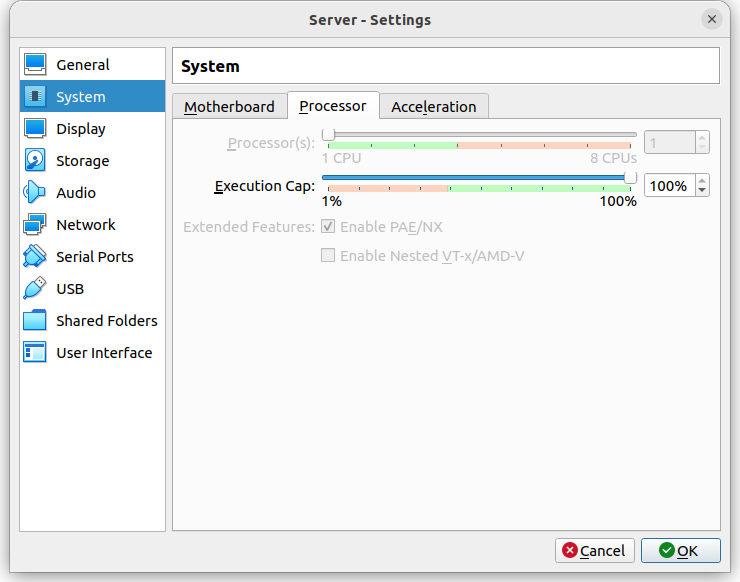
\includegraphics[width=12cm]{images/server-processor.png}
                        \caption{Số Core CPU cho Server}
                        \label{figure:server-processor}
                    \end{minipage}

                    \begin{minipage}{\linewidth}
                        \captionsetup{type=figure}
                        \centering
                        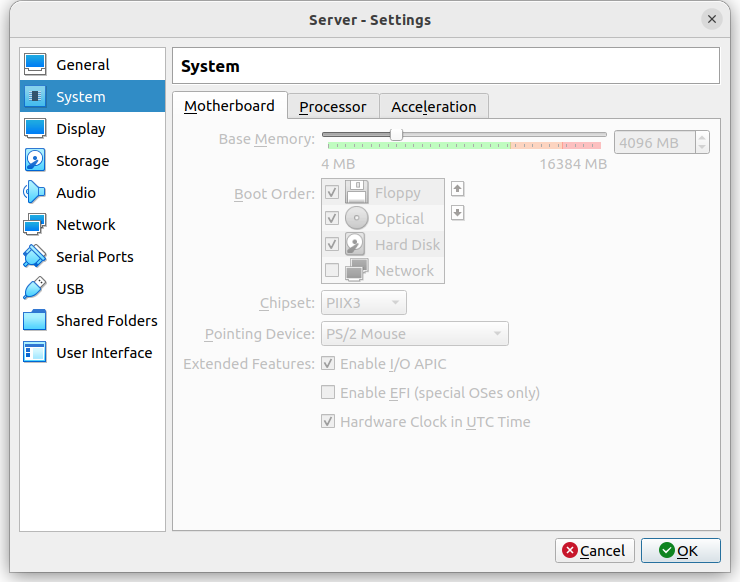
\includegraphics[width=12cm]{images/server-ram.png}
                        \caption{Dung lượng RAM cho Server}
                        \label{figure:server-ram}
                    \end{minipage}

                    \begin{minipage}
                        {\linewidth}
                        \captionsetup{type=figure}
                        \centering
                        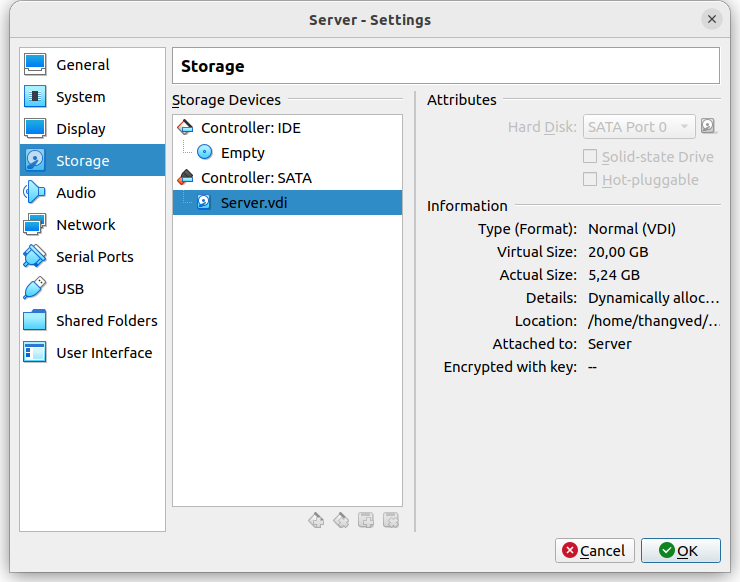
\includegraphics[width=12cm]{images/server-disk.png}
                        \caption{Dung lượng ổ cứng cho Server}
                        \label{figure:server-disk}
                    \end{minipage}

                    \begin{minipage}
                        {\linewidth}
                        \captionsetup{type=figure}
                        \centering
                        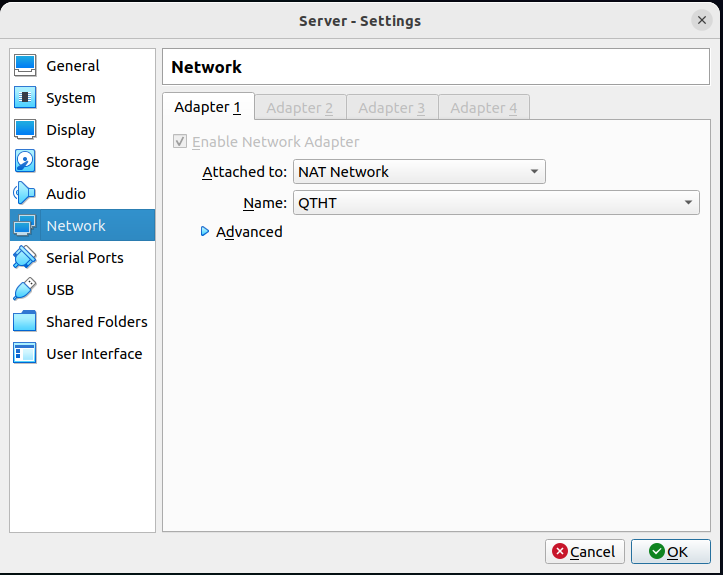
\includegraphics[width=12cm]{images/server-network-1.png}
                        \caption{Cấu hình mạng máy Server (1)}
                        \label{figure:server-network-1}
                    \end{minipage}

                    \begin{minipage}
                        {\linewidth}
                        \captionsetup{type=figure}
                        \centering
                        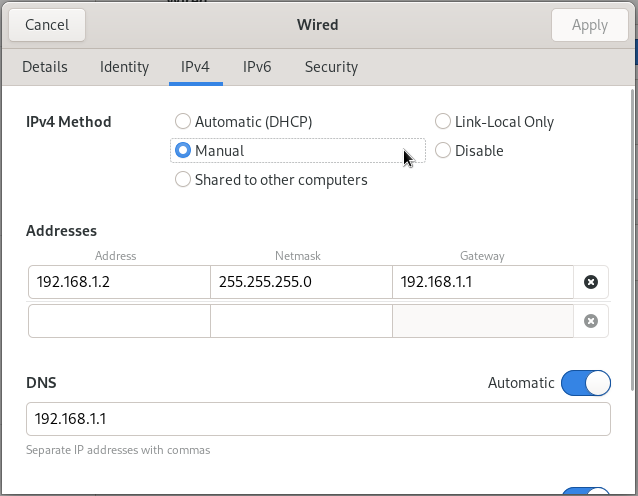
\includegraphics[width=12cm]{images/server-network-2.png}
                        \caption{Cấu hình mạng máy Server (2)}
                        \label{figure:server-network-2}
                    \end{minipage}

              \item \textbf{Máy Desktop có cấu hình như sau:}
                    \begin{itemize}
                        \item Hệ điều hành: Lubuntu 22.04.3 LTS (Jammy Jellyfish)
                        \item CPU: 1 Core \textit{(Hình \ref{figure:desktop-processor})}
                        \item Ram: 4GB \textit{(Hình \ref{figure:desktop-ram})}
                        \item Disk: 20GB \textit{(Hình \ref{figure:desktop-disk})}
                        \item Network: NAT Network "QTHT" \textit{(Hình \ref{figure:desktop-network})}
                    \end{itemize}

                    \begin{minipage}
                        {\linewidth}
                        \captionsetup{type=figure}
                        \centering
                        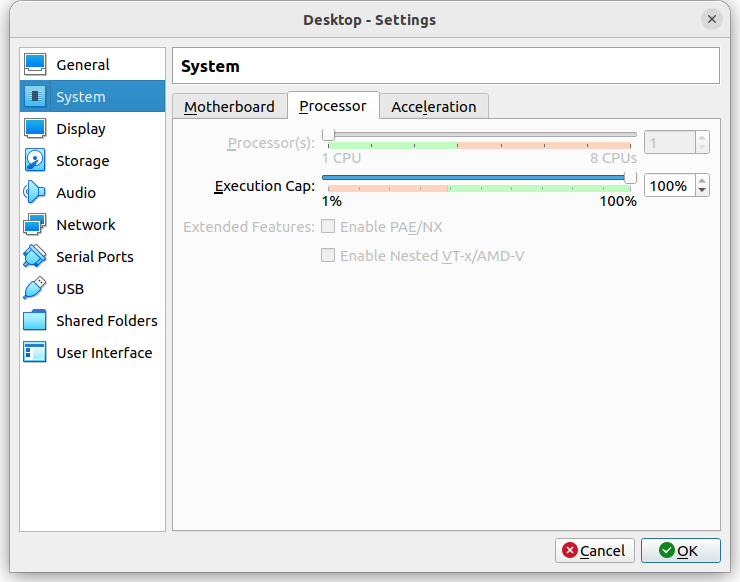
\includegraphics[width=12cm]{images/desktop-processor.png}
                        \caption{Số Core CPU cho máy Desktop}
                        \label{figure:desktop-processor}
                    \end{minipage}

                    \begin{minipage}
                        {\linewidth}
                        \captionsetup{type=figure}
                        \centering
                        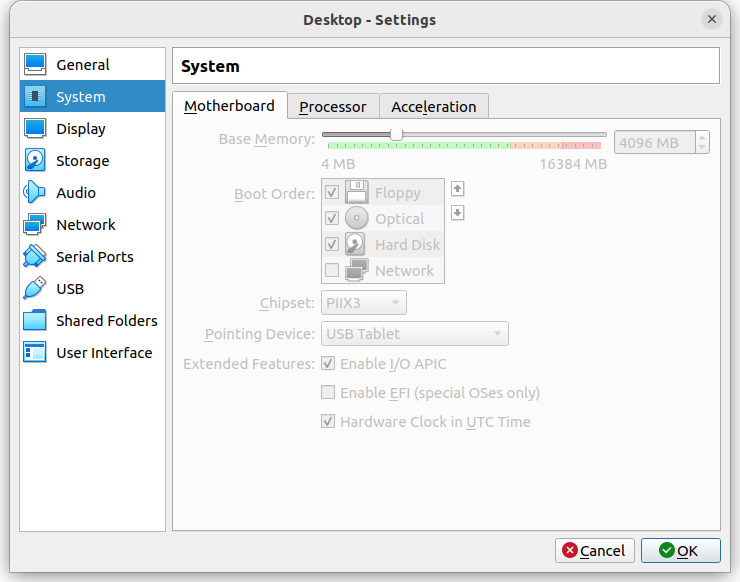
\includegraphics[width=12cm]{images/desktop-ram.png}
                        \caption{Dung lượng RAM cho máy Desktop}
                        \label{figure:desktop-ram}
                    \end{minipage}

                    \begin{minipage}
                        {\linewidth}
                        \captionsetup{type=figure}
                        \centering
                        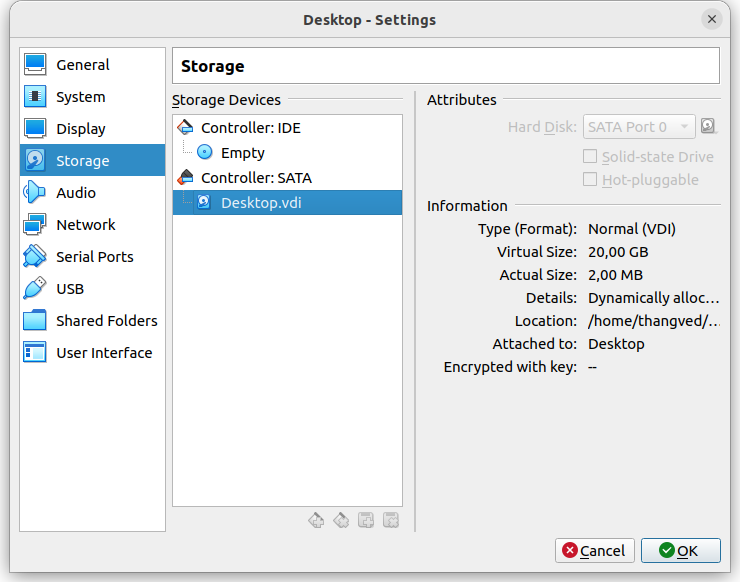
\includegraphics[width=12cm]{images/desktop-disk.png}
                        \caption{Dung lượng ổ đĩa cho máy Desktop}
                        \label{figure:desktop-disk}
                    \end{minipage}

                    \begin{minipage}
                        {\linewidth}
                        \captionsetup{type=figure}
                        \centering
                        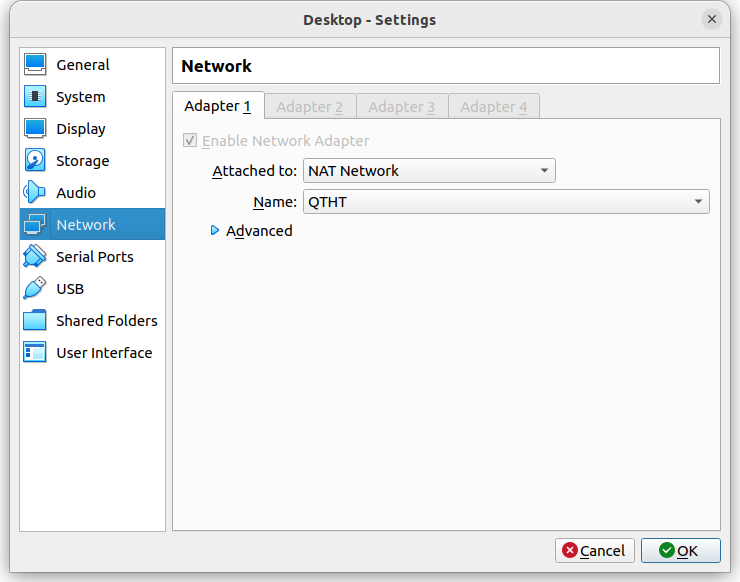
\includegraphics[width=12cm]{images/desktop-network.png}
                        \caption{Cấu hình mạng cho máy Desktop}
                        \label{figure:desktop-network}
                    \end{minipage}
          \end{enumerate}
    \item Trong quá trình cài hệ điều hành CentOS 9, tạo 1 tài khoản với username là <Mã số sinh viên>; firstname và lastname là họ tên của sinh viên. Cấp quyền quản trị (sudo) cho tài khoản. Sử dụng tài khoản vừa tạo để thực hiện bài tập tổng hợp (không dùng tài khoản root).
    \item Tắt dịch vụ tường lửa trên Server. \hfill \\
          Để tắt tường lửa ta có thể sử dụng lệnh \texttt{systemctl} hoặc \texttt{service}.
          Ở đây ta sẽ sử dụng lệnh \texttt{systemctl} để làm việc này \textit{(xem Hình \ref{figure:stop-firewalld}) và Hình \ref{figure:disable-firewalld}}. \\

          \begin{minipage}
              {\linewidth}
              \captionsetup{type=figure}
              \centering
              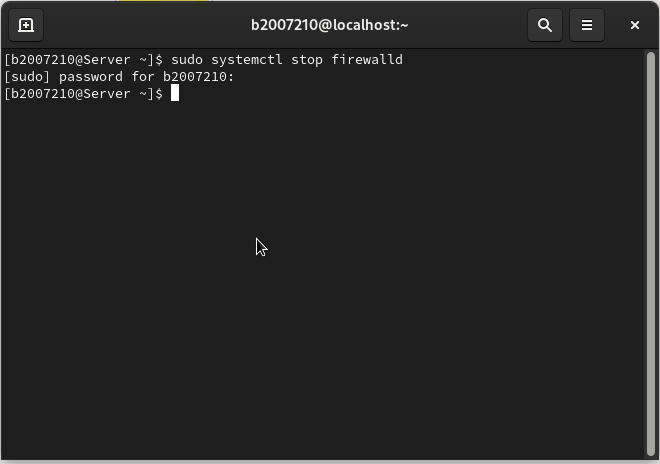
\includegraphics[width=12cm]{images/stop-firewalld.png}
              \caption{Dừng tường lửa bằng cách sử dụng \texttt{systemctl stop firewalld}}
              \label{figure:stop-firewalld}
          \end{minipage}

          \begin{lstlisting}[language=bash, caption=Dừng tường lửa]
sudo systemctl stop firewalld
\end{lstlisting}

          \begin{minipage}
              {\linewidth}
              \captionsetup{type=figure}
              \centering
              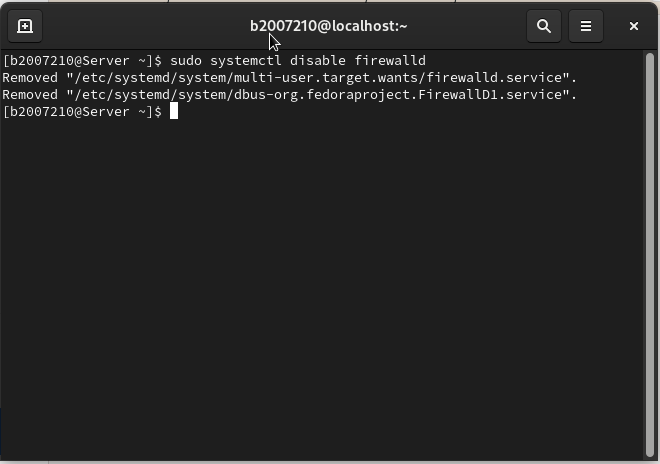
\includegraphics[width=12cm]{images/disable-firewalld.png}
              \caption{Ngăn tường lửa tự khởi động lại bằng cách sử dụng \texttt{systemctl disable firewalld}}
              \label{figure:disable-firewalld}
          \end{minipage}

          \begin{lstlisting}[language=bash, caption=Ngăn tường lửa tự khởi động lại]
sudo systemctl disable firewalld
\end{lstlisting}

          Lệnh \texttt{systemctl stop firewalld} \textit{(Hình \ref{figure:stop-firewalld})} dùng để dừng tường lửa ngay lập tức và lệnh \texttt{systemctl disable firewalld} \textit{(Hình \ref{figure:disable-firewalld})} sẽ ngăn việc tường lửa tự khởi động lại sau khi reboot.
\end{itemize}

\subsection{(10\%) Tạo các người dùng và nhóm người dùng}

Để quản lý các bộ phận và người dùng trong công ty, hãy tạo các nhóm người dùng (group) và người dùng (user) trên server như sau. Cấp quyền sudo cho người dùng Nami.

\begin{longtable}{|c|c|c|c|c|c|}
    \caption{Danh sách người dùng và nhóm người dùng}              \\
    \hline
    STT & Họ tên  & Nhóm       & Username & Pasword & Mô tả        \\
    \hline

    1   & Luffy   & bangiamdoc & luffy    & luffy   & Giám đốc     \\
    \hline

    2   & Nami    & bangiamdoc & nami     & nami    & Phó giám đốc \\
    \hline

    3   & Zoro    & banhang    & zoro     & zoro    & Trưởng phòng \\
    \hline

    4   & Usopp   & banhang    & usopp    & usopp   & Nhân viên    \\
    \hline

    5   & Robin   & banhang    & robin    & robin   & Nhân viên    \\
    \hline

    6   & Sanji   & hanhchinh  & sanji    & sanji   & Trưởng phòng \\
    \hline

    7   & Chopper & hanhchinh  & chopper  & chopper & Nhân viên    \\
    \hline
\end{longtable}

Để tạo người dùng trên CentOS, ta có thể sử dụng lệnh \texttt{useradd <username>} và dùng lệnh \texttt{passwd <username>} để đặt mật khẩu cho user.
Sau đây là ví dụ về việc tạo tài khoản và đặt mật khẩu cho tài khoản luffy \textit{(Hình \ref{figure:useradd-luffy})}.

\begin{minipage}
    {\linewidth}
    \captionsetup{type=figure}
    \centering
    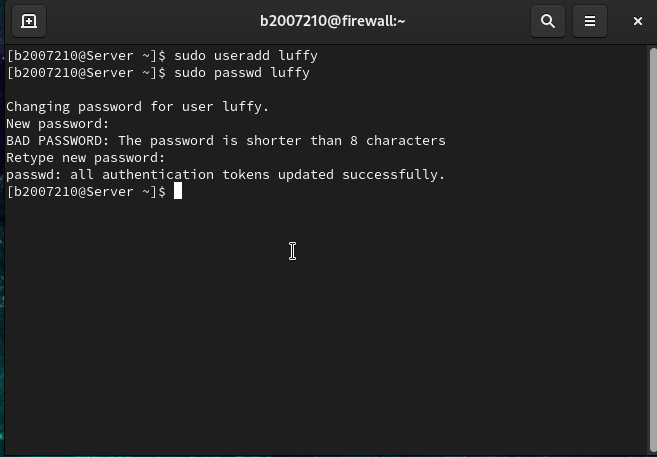
\includegraphics[width=12cm]{images/useradd-luffy.png}
    \caption{Tạo và đặt mật khẩu cho tài khoản luffy}
    \label{figure:useradd-luffy}
\end{minipage}

\begin{lstlisting}[language=bash, caption=Tạo và đặt mật khẩu cho tài khoản luffy]
sudo useradd luffy
sudo passwd luffy
\end{lstlisting}

Tương tự như thế với các tài khoản còn lại \textit{(Hình \ref{figure:useradd-other})}.

\begin{minipage}
    {\linewidth}
    \captionsetup{type=figure}
    \centering
    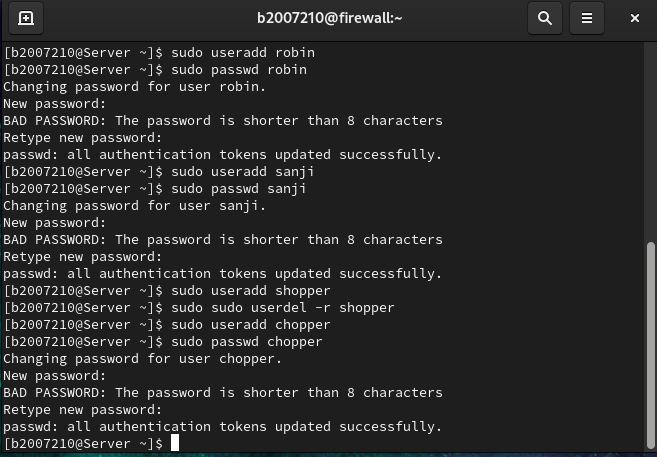
\includegraphics[width=12cm]{images/useradd-other.png}
    \caption{Tạo và đặt mật khẩu cho các người dùng còn lại}
    \label{figure:useradd-other}
\end{minipage}

\begin{lstlisting}[language=bash, caption=Tạo và đặt mật khẩu cho các người dùng còn lại]
sudo useradd nami
sudo passwd nami
sudo useradd zoro
sudo passwd zoro
sudo useradd usopp
sudo passwd usopp
sudo useradd robin
sudo passwd robin
sudo useradd sanji
sudo passwd sanji
sudo useradd chopper
sudo passwd chopper
\end{lstlisting}

Để thêm nhóm người dùng, ta sử dụng lệnh \texttt{groupadd <group-name>} và thêm người dùng vào nhóm bằng lệnh \texttt{usermod -aG <group-name> <username>}.
Sau đây là ví dụ tạo nhóm \texttt{bangiamdoc} và thêm \texttt{luffy} và \texttt{nami} vào nhóm này \textit{(Hình \ref{figure:groupadd-bangiamdoc})}.

\begin{minipage}
    {\linewidth}
    \captionsetup{type=figure}
    \centering
    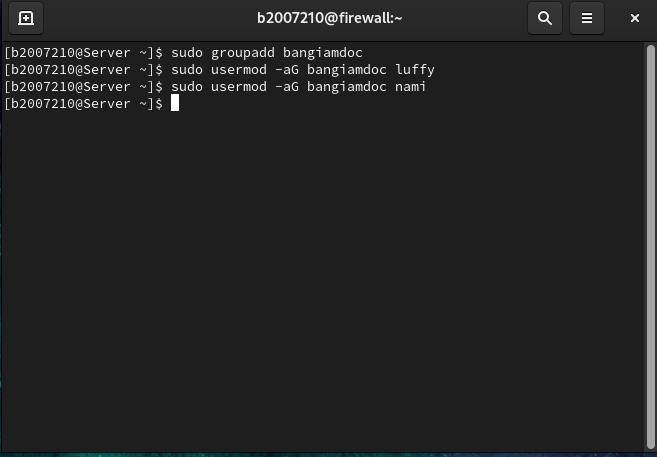
\includegraphics[width=12cm]{images/groupadd-bangiamdoc.png}
    \caption{Tạo nhóm bangiamdoc và thêm người dùng vào}
    \label{figure:groupadd-bangiamdoc}
\end{minipage}

\begin{lstlisting}[language=bash, caption=Tạo nhóm \texttt{bangiamdoc} và thêm người dùng vào]
sudo groupadd bangiamdoc
sudo usermod -aG bangiamdoc luffy
sudo usermod -aG bangiamdoc nami
\end{lstlisting}

Thực hiện tương tự với các nhóm còn lại \textit{(Hình \ref{figure:groupadd-other})}.

\begin{minipage}
    {\linewidth}
    \captionsetup{type=figure}
    \centering
    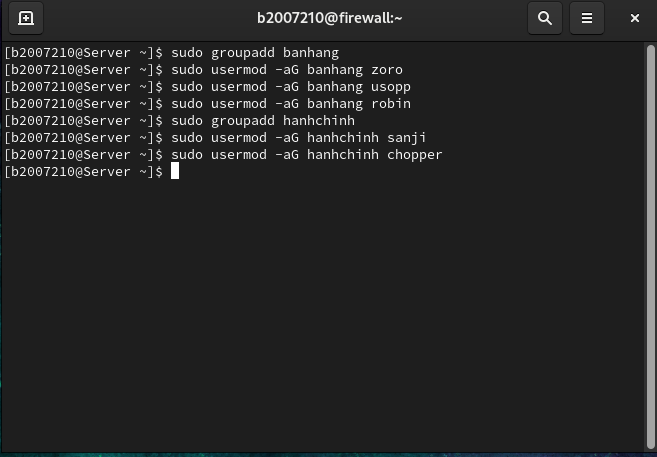
\includegraphics[width=12cm]{images/groupadd-other.png}
    \caption{Tạo các nhóm còn lại và thêm người dùng vào}
    \label{figure:groupadd-other}
\end{minipage}

\begin{lstlisting}[language=bash, caption=Tạo các nhóm còn lại và thêm người dùng vào]
sudo groupadd banhang
sudo usermod -aG banhang zoro
sudo usermod -aG banhang usopp
sudo usermod -aG banhang robin

sudo groupadd hanhchinh
sudo usermod -aG hanhchinh sanji
sudo usermod -aG hanhchinh chopper
\end{lstlisting}

Để cấp quyền sudo cho một user, ta chỉ cần thêm user đó vào nhóm \texttt{sudo} hoặc \texttt{wheel}.
Trong trường hợp này, ta sẽ thêm vào nhóm \texttt{wheel}.

\begin{minipage}
    {\linewidth}
    \captionsetup{type=figure}
    \centering
    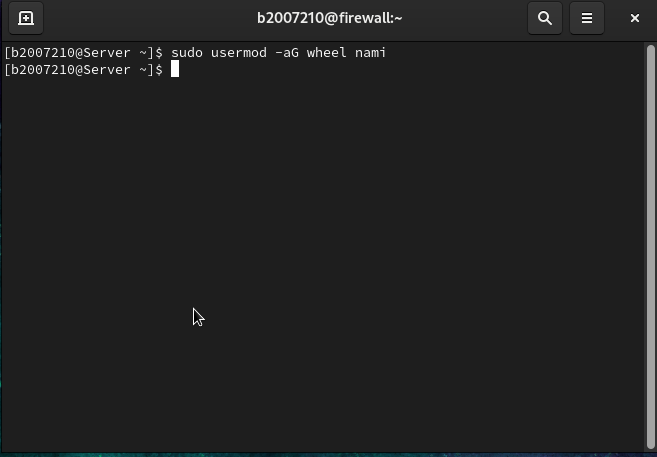
\includegraphics[width=12cm]{images/wheel-nami.png}
    \caption{Cấp quyền sudo cho user nami}
    \label{figure:wheel-nami}
\end{minipage}

\begin{lstlisting}[language=bash, caption=Cấp quyền sudo cho user nami]
sudo usermod -aG wheel nami
\end{lstlisting}

\subsection{(10\%)  Cài đặt và cấu hình dịch vụ SSH để cho phép điều khiển từ xa Server}

\begin{itemize}
    \item Chỉ có thành viên ban giám đốc và tài khoản <Mã số sinh viên> mới có quyền điều khiển từ xa Server. Tài khoản root không được nối kết tới server từ xa.
    \item Chỉ cho phép chứng thực bằng private key, không cho phép chứng thực bằng password. Tạo private/public key cho người dùng <Mã số sinh viên> để có thể SSH tới server.
\end{itemize}

\begin{enumerate}
    \item Cài đặt dịch vụ ssh \hfill \\
          \begin{minipage}
              {\linewidth}
              \captionsetup{type=figure}
              \centering
              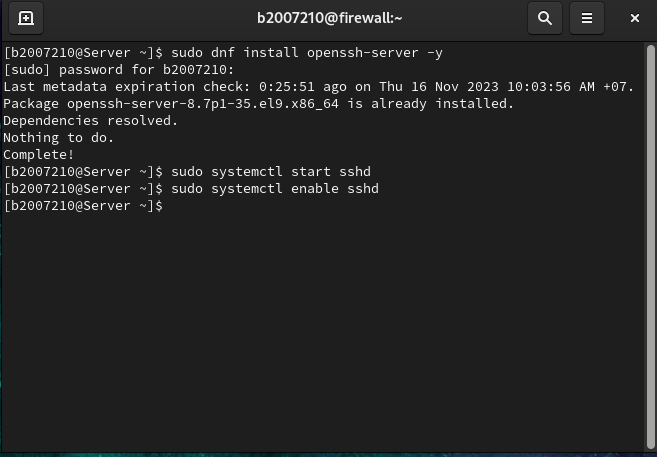
\includegraphics[width=12cm]{images/install-ssh.png}
              \caption{Cài đặt và kích hoạt dịch vụ ssh}
              \label{figure:install-ssh}
          \end{minipage}
          \begin{lstlisting}[language=bash, caption=Cài đặt và kích hoạt dịch vụ ssh]
sudo dnf install openssh-server
sudo systemctl enable sshd
sudo systemctl start sshd
\end{lstlisting}
    \item Cấu hình chỉ cho phép thành viên trong ban giám đốc và tài khoản \texttt{b2007210} mới có quyền điều khiển từ xa \hfill \\
          Để cấu hình chỉ cho phép một nhóm người dùng hoặc người dùng có thể sử dụng dịch vụ ssh, ta sẽ cấu hình trong file \texttt{/etc/ssh/sshd\_config} \textit{(Hình \ref{figure:allow-groups-users})}. \\
          \begin{minipage}
              {\linewidth}
              \captionsetup{type=figure}
              \centering
              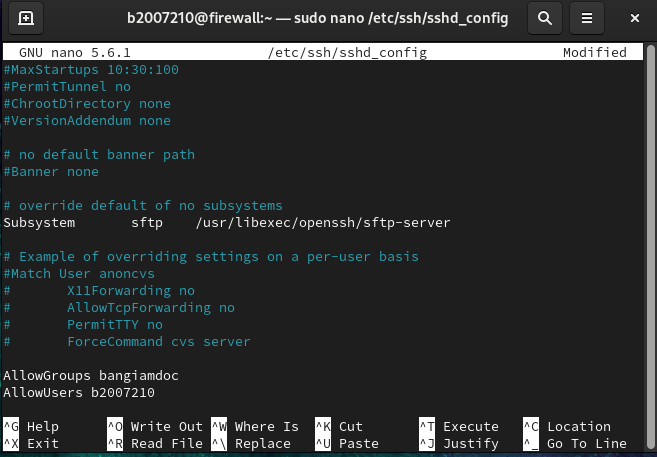
\includegraphics[width=12cm]{images/allow-groups-users.png}
              \caption{Cho phép nhóm \texttt{bangiamdoc} và user \texttt{b2007210} có quyền điều khiển máy tính từ xa}
              \label{figure:allow-groups-users}
          \end{minipage}
          \begin{itemize}
              \item \texttt{AllowGroups bangiamdoc}: Cho phép nhóm \texttt{bangiamdoc} sử dụng dịch vụ ssh.
              \item \texttt{AllowUsers b2007210}: Cho phép user \texttt{b2007210} sử dụng dịch vụ ssh.
          \end{itemize}

          Ta cần khởi động lại dịch vụ ssh để áp dụng những thay đổi này (dùng lệnh \texttt{systemctl restart sshd}).
    \item Chỉ cho phép chứng thực bằng private key \hfill \\
          Để cấu hình chỉ cho phép chứng thực bằng private key, ta sẽ cấu hình trong file \texttt{/etc/ssh/sshd\_config} \textit{(Hình \ref{figure:ssh-only-pubkey})}. \\
          \begin{minipage}
              {\linewidth}
              \captionsetup{type=figure}
              \centering
              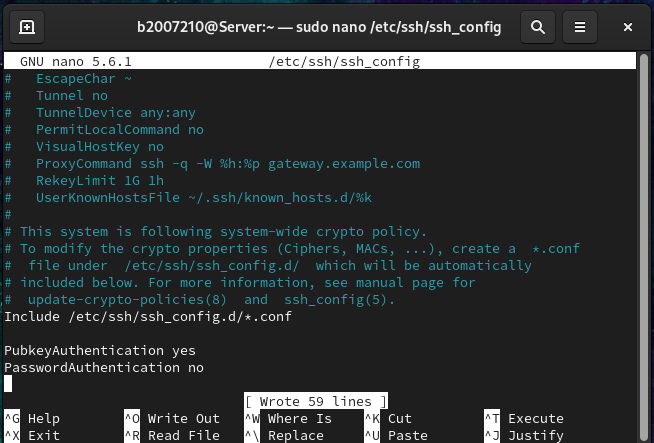
\includegraphics[width=12cm]{images/ssh-only-pubkey.png}
              \caption{Cấu hình cho phép truy cập dịch vụ ssh bằng private key}
              \label{figure:ssh-only-pubkey}
          \end{minipage}
          \begin{itemize}
              \item \texttt{\textbf{PubkeyAuthentication} yes}: Cho phép chứng thực bằng private key.
              \item \texttt{\textbf{PasswordAuthentication} no}: Không cho phép chứng thực bằng password.
          \end{itemize}
          Sau khi cấu hình xong, ta cần khởi động lại dịch vụ ssh để áp dụng những thay đổi này (dùng lệnh \texttt{systemctl restart sshd}).

          Để tạo private key và public key, ta sử dụng lệnh \texttt{ssh-keygen} \textit{(Hình \ref{figure:ssh-keygen})}. \\
          \begin{minipage}
              {\linewidth}
              \captionsetup{type=figure}
              \centering
              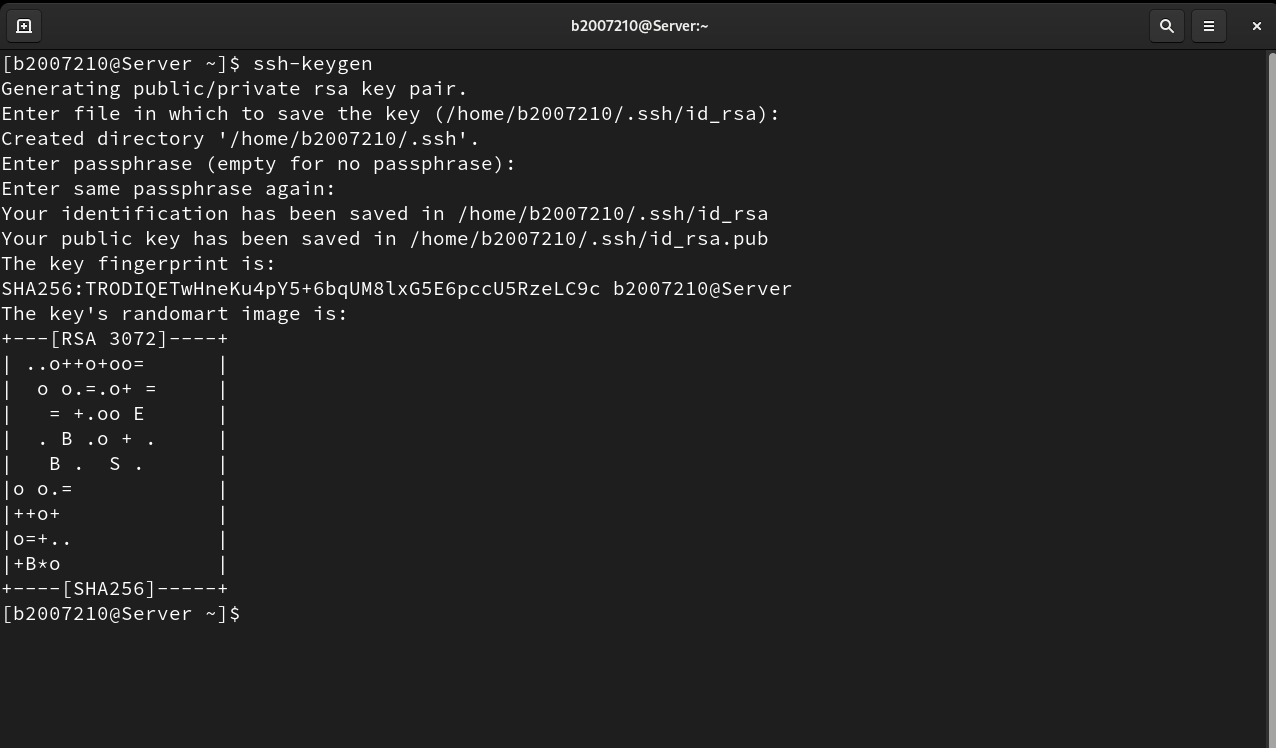
\includegraphics[width=12cm]{images/ssh-keygen.png}
              \caption{Tạo private key và public key}
              \label{figure:ssh-keygen}
          \end{minipage}

          Sau đó, ta cần đổi lại tên của public key thành \texttt{authorized\_keys} và phân lại quyền cho tập tin này \textit{(Hình \ref{figure:rename-authorized-keys})}. \\
          \begin{minipage}
              {\linewidth}
              \captionsetup{type=figure}
              \centering
              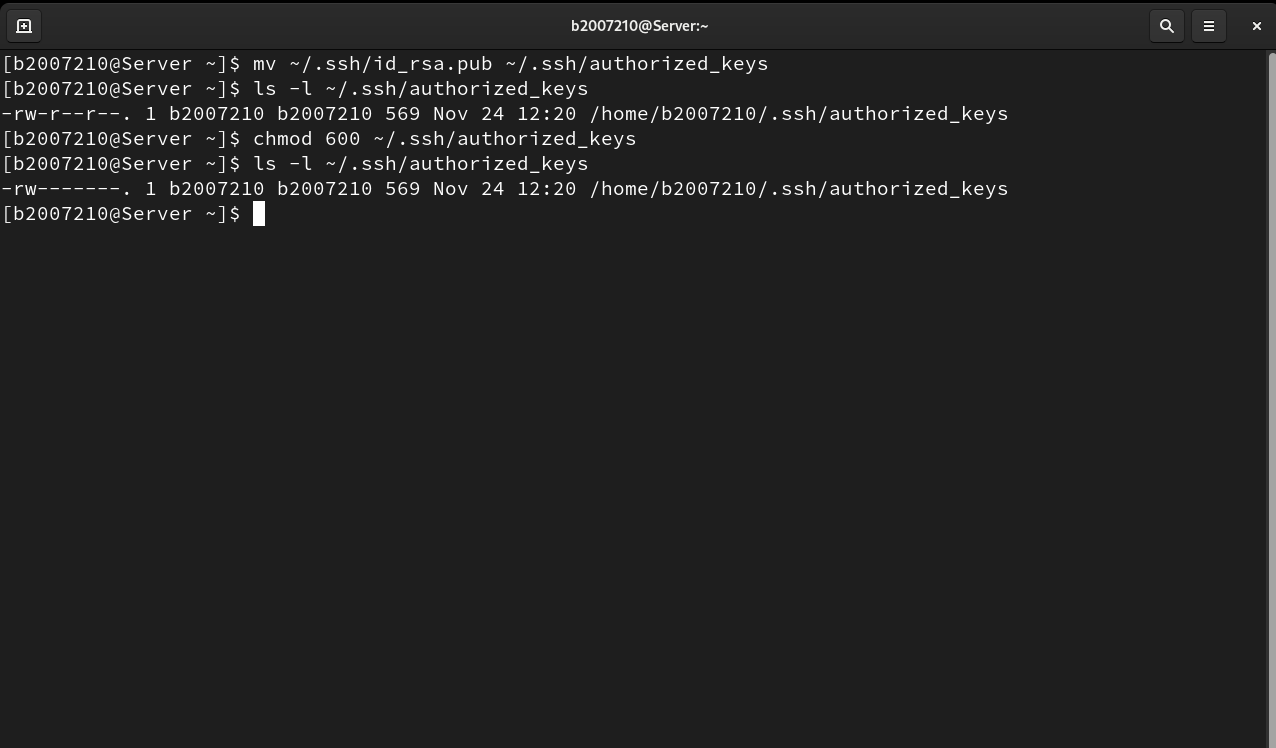
\includegraphics[width=12cm]{images/rename-authorized-keys.png}
              \caption{Đổi tên và phân quyền cho tập tin public key}
              \label{figure:rename-authorized-keys}
          \end{minipage}

          \begin{itemize}
              \item \texttt{mv \textasciitilde/.ssh/id\_rsa.pub \textasciitilde/.ssh/authorized\_keys}: Đổi tên tập tin public key thành \texttt{authorized\_keys}.
              \item \texttt{chmod 600 \textasciitilde/.ssh/authorized\_keys}: Cho phép chủ sở hữu đọc và ghi vào tập tin \texttt{authorized\_keys}.
          \end{itemize}
\end{enumerate}

\subsection{(10\%) Tạo và phân quyền cho thư mục \texttt{/data}}

Tạo thư mục /data trên server và phân quyền sao cho thành viên ban giám đốc có toàn quyền (read, write và execute), các trưởng phòng có quyền read và execute, các nhân viên không có bất cứ quyền gì. Ngoài ra chỉ chủ sở hữu tập tin có quyền xóa hoặc đổi tên tập tin trong thư mục /data.


Để tạo và phân quyền cho thư mục \texttt{/data}, ta thực hiện theo các bước như \textit{Hình \ref{figure:facl}}.

\begin{minipage}
    {\linewidth}
    \captionsetup{type=figure}
    \centering
    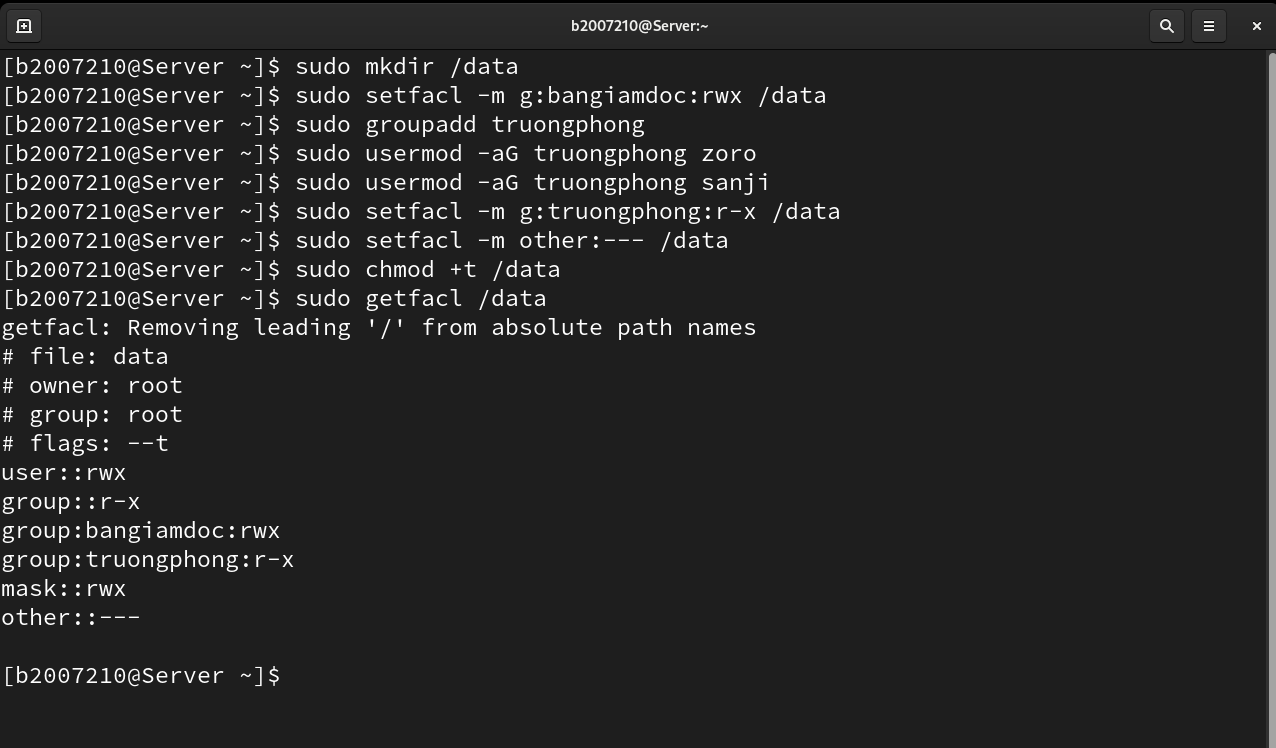
\includegraphics[width=12cm]{images/facl.png}
    \caption{Tạo và phân quyền cho thư mục \texttt{/data}}
    \label{figure:facl}
\end{minipage}

Cụ thể như sau:
\begin{enumerate}
    \item Tạo thư mục \texttt{/data}.
          \begin{lstlisting}[language=bash, caption=Tạo thư mục \texttt{/data}]
sudo mkdir /data
\end{lstlisting}
    \item \textbf{Ban giám đốc} có toàn quyền (read, write, execute) trên thư mục \texttt{/data}
          \begin{lstlisting}[language=bash, caption=Phân quyền cho ban giám đốc]
sudo setfacl -m g:bangiamdoc:rwx /data
\end{lstlisting}
    \item  \textbf{Trưởng phòng} có quyền read và execute trên thư mục \texttt{/data}
          \begin{lstlisting}[language=bash, caption=Phân quyền cho trưởng phòng]
sudo groupadd truongphong
sudo usermod -aG truongphong zoro
sudo usermod -aG truongphong sanji
sudo setfacl -m g:truongphong:rx /data
\end{lstlisting}

          \begin{itemize}
              \item [Dòng 1] Tạo nhóm \texttt{truongphong}.
              \item [Dòng 2] Thêm user \texttt{zoro} vào nhóm \texttt{truongphong}.
              \item [Dòng 3] Thêm user \texttt{sanji} vào nhóm \texttt{truongphong}.
              \item [Dòng 4] Phân quyền cho nhóm \texttt{truongphong} có quyền read và execute trên thư mục \texttt{/data}.
          \end{itemize}
    \item \textbf{Nhân viên} không có bất cứ quyền gì trên thư mục \texttt{/data}
          \begin{lstlisting}[language=bash, caption=Phân quyền cho nhân viên]
sudo setfacl -m other:--- /data
\end{lstlisting}
    \item Chỉ chủ sở hữu tập tin có quyền xóa hoặc đổi tên tập tin trong thư mục \texttt{/data}
          \begin{lstlisting}
sudo chmod +t /data
\end{lstlisting}
\end{enumerate}

\subsection{(5\%) Cài đặt và cấu hình tường lửa trên Server}

Có thể truy cập các dịch vụ DNS, DHCP, SSH, Web, SAMBA trên Server. Các dịch vụ khác KHÔNG cập truy cập được.

Ta sẽ cấu hình như \textit{Hình \ref{figure:config-firewall}}.

\begin{minipage}
    {\linewidth}
    \captionsetup{type=figure}
    \centering
    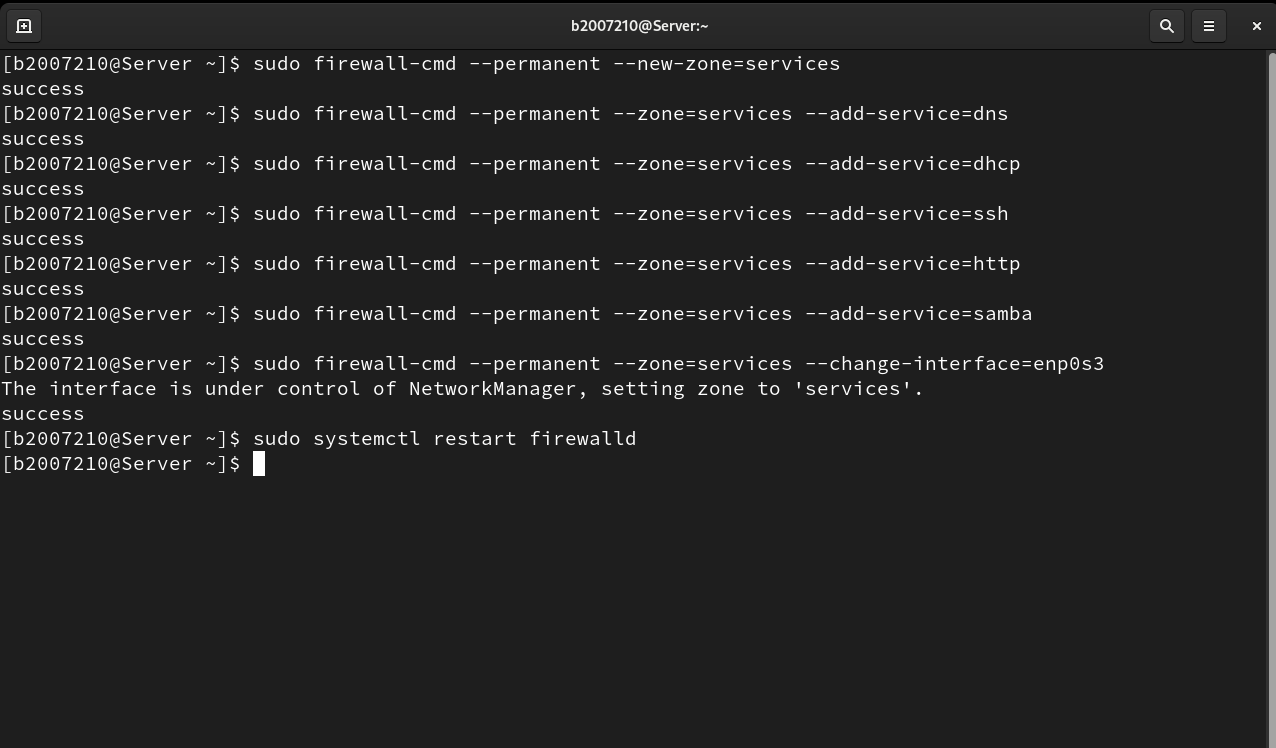
\includegraphics[width=12cm]{images/config-firewall.png}
    \caption{Cấu hình tường lửa trên Server}
    \label{figure:config-firewall}
\end{minipage}

Cụ thể như sau:
\begin{enumerate}
    \item Tạo một zone mới có tên là \texttt{services}
          \begin{lstlisting}[language=bash, caption=Tạo zone mới có tên là \texttt{services}]
sudo firewall-cmd --permanent --new-zone=services
\end{lstlisting}
    \item Thêm các dịch vụ DNS, DHCP, SSH, Web, SAMBA vào zone \texttt{services}
          \begin{lstlisting}[language=bash, caption={Thêm các dịch vụ DNS, DHCP, SSH, Web, SAMBA vào zone \texttt{services}}]
sudo firewall-cmd --permanent --zone=services --add-service=dns
sudo firewall-cmd --permanent --zone=services --add-service=dhcp
sudo firewall-cmd --permanent --zone=services --add-service=ssh
sudo firewall-cmd --permanent --zone=services --add-service=http
sudo firewall-cmd --permanent --zone=services --add-service=samba
\end{lstlisting}
    \item Khởi động lại dịch vụ tường lửa để áp dụng những thay đổi này
          \begin{lstlisting}
sudo systemctl restart firewalld
\end{lstlisting}
\end{enumerate}

\end{document}